%\title{LaTeX Portrait Poster Template}
%%%%%%%%%%%%%%%%%%%%%%%%%%%%%%%%%%%%%%%%%
% a0poster Portrait Poster
% LaTeX Template
% Version 1.0 (22/06/13)
%
% The a0poster class was created by:
% Gerlinde Kettl and Matthias Weiser (tex@kettl.de)
% 
% This template has been downloaded from:
% http://www.LaTeXTemplates.com
%
% License:
% CC BY-NC-SA 3.0 (http://creativecommons.org/licenses/by-nc-sa/3.0/)
%
%%%%%%%%%%%%%%%%%%%%%%%%%%%%%%%%%%%%%%%%%

%----------------------------------------------------------------------------------------
%	PACKAGES AND OTHER DOCUMENT CONFIGURATIONS
%----------------------------------------------------------------------------------------

\documentclass[a0,portrait]{a0poster}

\usepackage{multicol} % This is so we can have multiple columns of text side-by-side
\columnsep=100pt % This is the amount of white space between the columns in the poster
\columnseprule=3pt % This is the thickness of the black line between the columns in the poster

\usepackage[svgnames]{xcolor} % Specify colors by their 'svgnames', for a full list of all colors available see here: http://www.latextemplates.com/svgnames-colors

\usepackage{times} % Use the times font
%\usepackage{palatino} % Uncomment to use the Palatino font

\usepackage{graphicx} % Required for including images
\graphicspath{{figures/}} % Location of the graphics files
\usepackage{booktabs} % Top and bottom rules for table
\usepackage[font=small,labelfont=bf]{caption} % Required for specifying captions to tables and figures
\usepackage{amsfonts, amsmath, amsthm, amssymb} % For math fonts, symbols and environments
\usepackage{wrapfig} % Allows wrapping text around tables and figures

\begin{document}

%----------------------------------------------------------------------------------------
%	POSTER HEADER 
%----------------------------------------------------------------------------------------

% The header is divided into two boxes:
% The first is 75% wide and houses the title, subtitle, names, university/organization and contact information
% The second is 25% wide and houses a logo for your university/organization or a photo of you
% The widths of these boxes can be easily edited to accommodate your content as you see fit

% full affiliation list
% \newcommand{\Bern}{Institute for Theoretical Physics, Albert Einstein Center for Fundamental Physics,\\University of Bern, Sidlerstrasse 5, CH-3012 Bern, Switzerland}
% \newcommand{\hiskp}{HISKP (Theory), Rheinische Friedrich-Wilhelms-Universit\"at Bonn,\\Nussallee 14-16, 53115 Bonn, Germany}
% \newcommand{\hpca}{High Performance Computing and Analytics Lab, Rheinische Friedrich-Wilhelms-Universit\"at Bonn,\\ Friedrich-Hirzebruch-Allee 8, 53115 Bonn, Germany}
% \newcommand{\CyprusU}{Department of Physics, University of Cyprus, 20537 Nicosia, Cyprus}
% \newcommand{\CyprusI}{Computation-based Science and Technology Research Center, The Cyprus Institute,\\20 Konstantinou Kavafi Street, 2121 Nicosia, Cyprus}
% \newcommand{\Jena}{University of Jena, Institute for Theoretical Physics, Max-Wien-Platz 1, D-07743 Jena, Germany}
% \newcommand{\Parma}{Dipartimento  di  Scienze  Matematiche,  Fisiche  e  Informatiche,  Universit\`a  di  Parma  and  INFN, Gruppo  Collegato  di  Parma,  Parco  Area  delle  Scienze  7/a  (Campus),  43124  Parma,  Italy}
% \newcommand{\Romadue}{Dipartimento di Fisica and INFN, Universit\`a di Roma ``Tor Vergata",\\Via della Ricerca Scientifica 1, I-00133 Roma, Italy}
% \newcommand{\Romatre}{Dipartimento di Matematica e Fisica, Universit\`a Roma Tre and INFN, Sezione di Roma Tre,\\Via della Vasca Navale 84, I-00146 Rome, Italy}
% \newcommand{\RomatreINFN}{Istituto Nazionale di Fisica Nucleare, Sezione di Roma Tre,\\Via della Vasca Navale 84, I-00146 Rome, Italy}
% \newcommand{\NIC}{NIC, DESY, Platanenallee 6, D-15738 Zeuthen, Germany}
% \newcommand{\Berlin}{Institut f\"ur Physik, Humboldt-Universit\"at zu Berlin, Newtonstrasse 15, 12489 Berlin, Germany}

\begin{minipage}[b]{0.74\linewidth}
    \VeryHuge \color{NavyBlue} \textbf{Status of the ETMC ensemble generation effort} \color{Black}\\[1.4cm] % Title
    % \Huge\textit{Subtitle}\\[2.4cm] % Subtitle
    \Large \textbf{A.~Constantia$^{a)b)}$, B.~Simone$^{b)}$, F.~Jacob$^{c)}$, F,~Roberto$^{d)}$ M.~Garofalo$^{e)}$, B.~Kostrzewa$^{f)}$, K.~Giannis$^{b)}$, R.~Simone$^{g)}$, U.~Carsten$^{e)}$, W.~Urs$^{g)}$}\\[0.5cm] % Author(s)
    \large $^{a)}$ Department of Physics, University of Cyprus, 20537 Nicosia, Cyprus\\
    \large $^{b)}$ Computation-based Science and Technology Research Center, The Cyprus Institute, 2121 Nicosia, Cyprus\\
    \large $^{c)}$ Theoretical Physics Department, CERN 1211 Geneva 23, Switzerland\\
    \large $^{d)}$ Dipartimento di Fisica and INFN, Universit\`a di Roma ``Tor Vergata", I-00133 Roma, Italy\\
    \large $^{e)}$ Helmholtz-Institut f{\"u}r Strahlen- und Kernphysik (Theorie), University of Bonn, 53115 Bonn, Germany\\
    \large $^{f)}$ High Performance Computing and Analytics Lab, University of Bonn, 53115 Bonn, Germany\\
    \large $^{g)}$  Institute for Theoretical Physics, Albert Einstein Center for Fundamental Physics, University of Bern, CH-3012 Bern, Switzerland\\
\end{minipage}
%
\begin{minipage}[b]{0.26\linewidth}
    % \includegraphics[width=7cm]{logo.png}\ 
    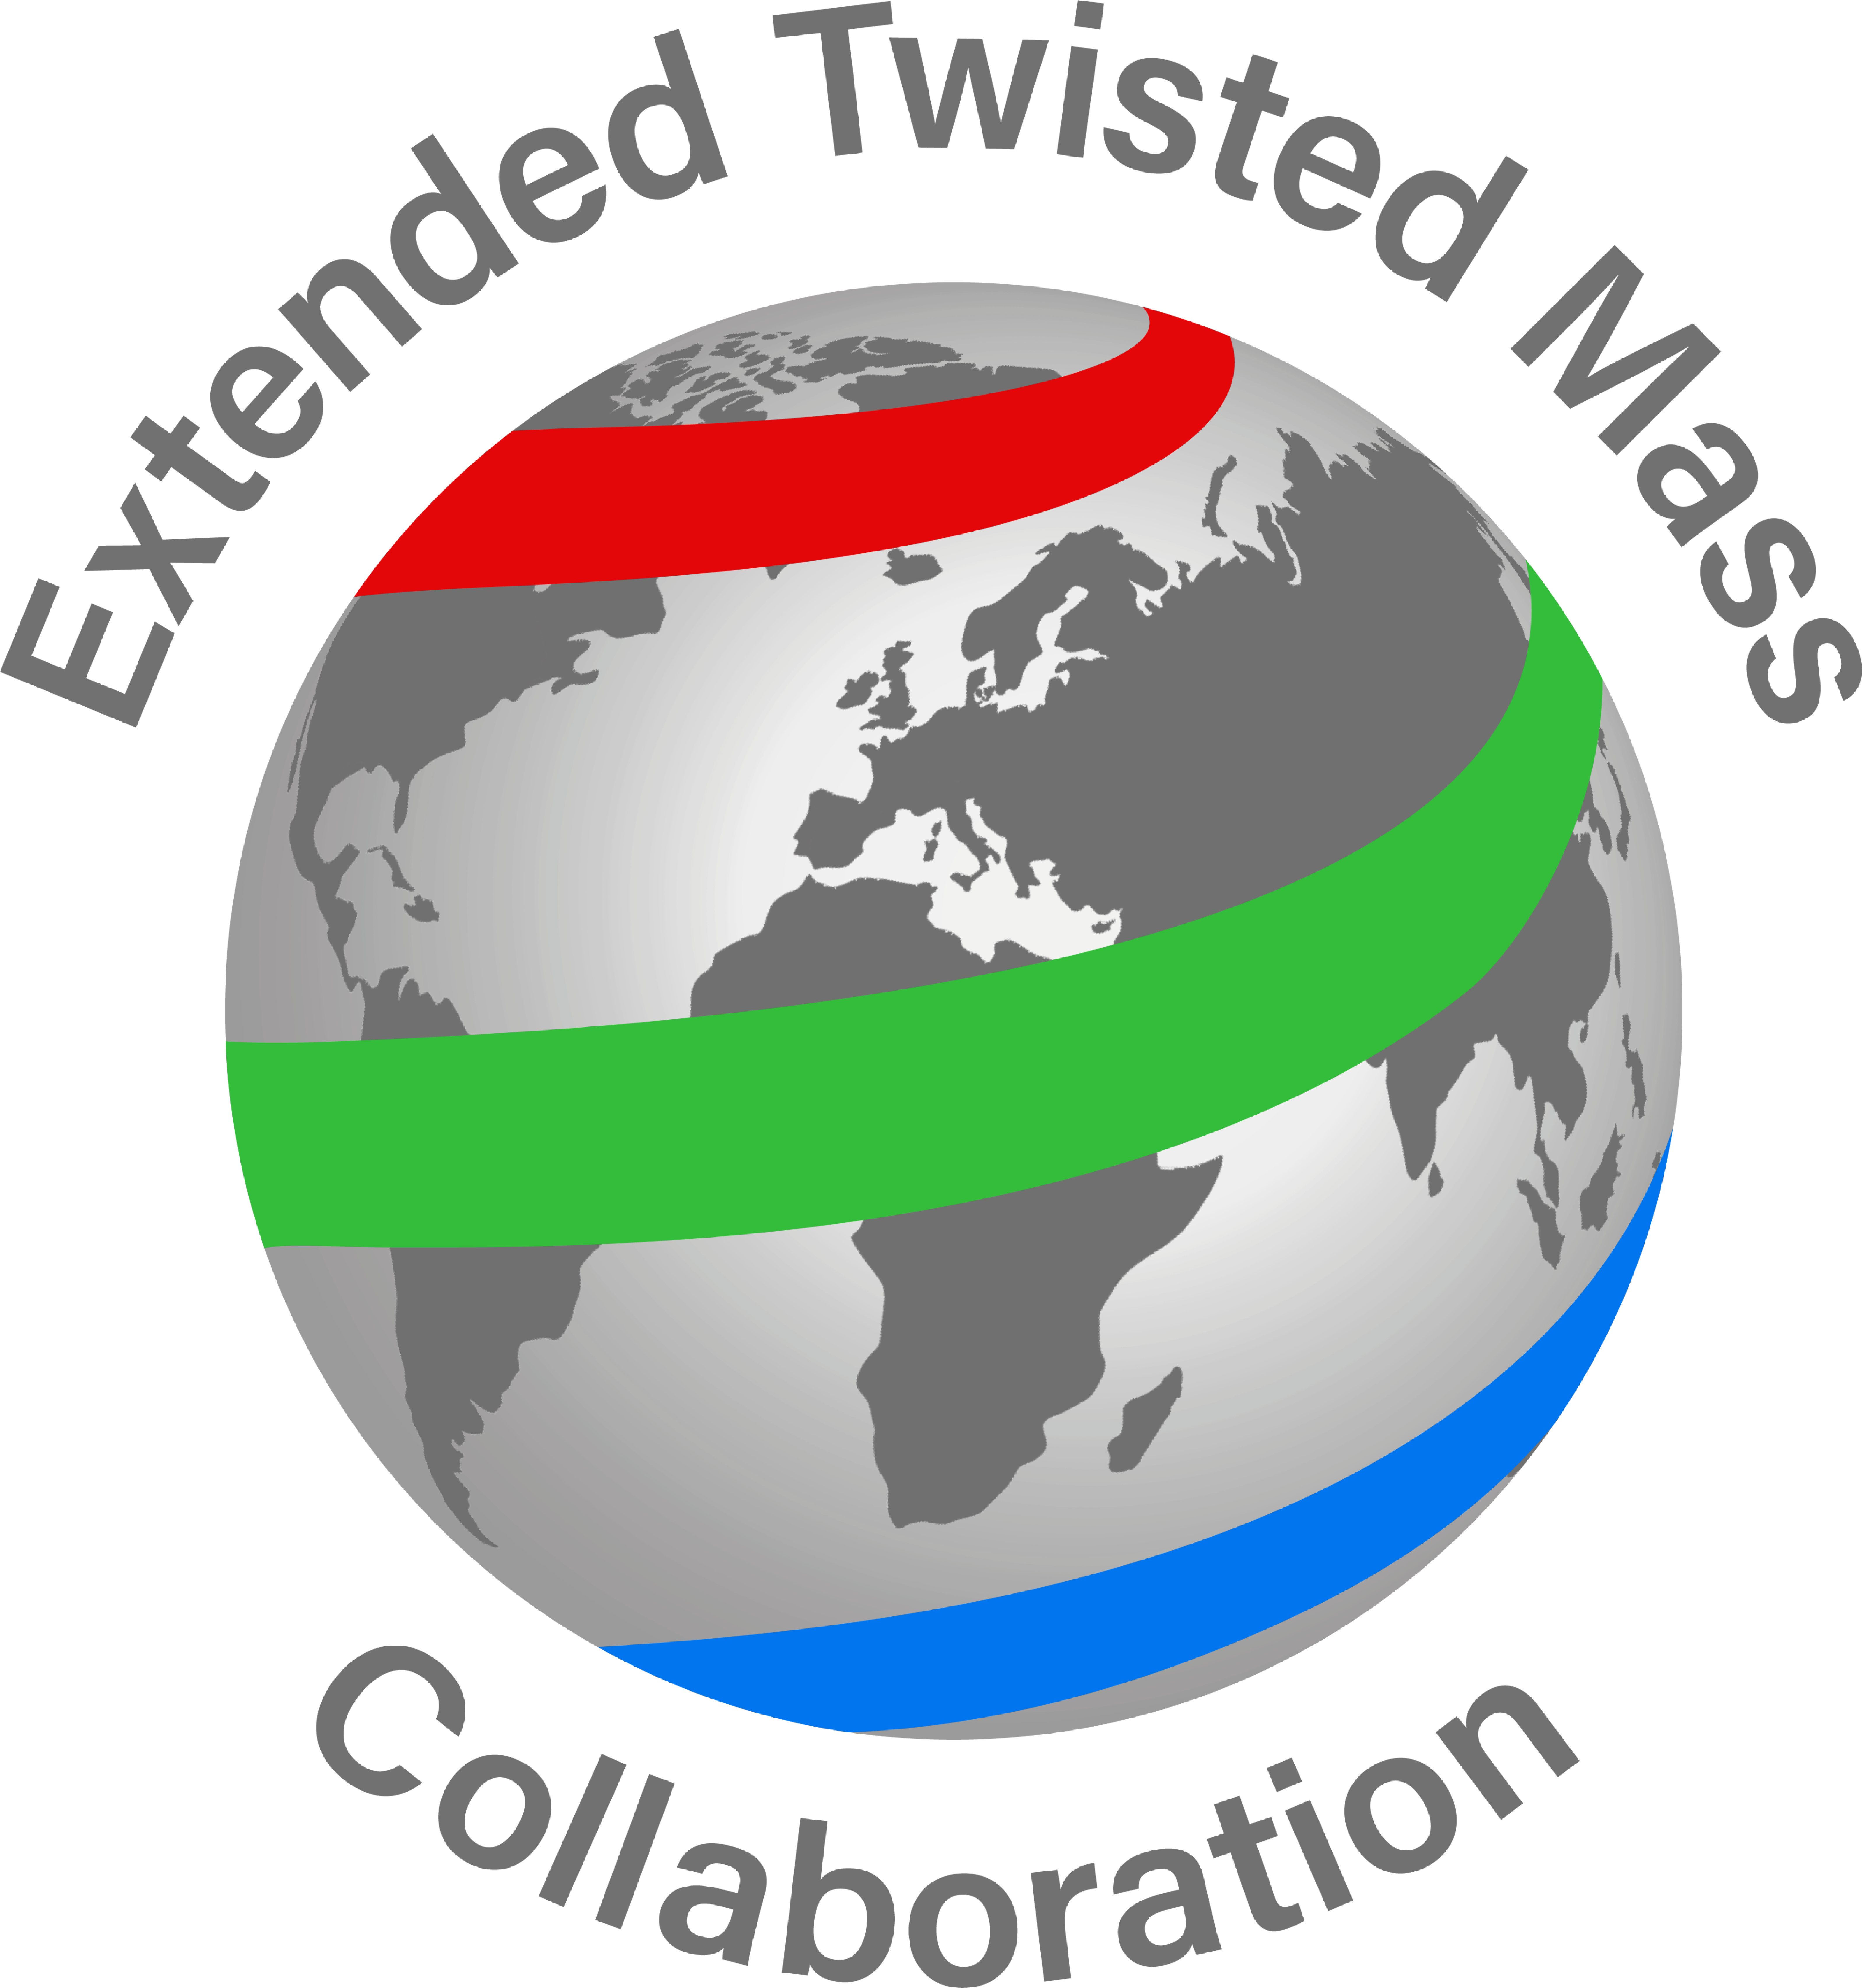
\includegraphics[width=14cm]{figures/Logo_ETMC_RGB.pdf}
\end{minipage}

\vspace{1cm} % A bit of extra whitespace between the header and poster content

%----------------------------------------------------------------------------------------

\begin{multicols}{2} % This is how many columns your poster will be broken into, a portrait poster is generally split into 2 columns

    %----------------------------------------------------------------------------------------
    %	ABSTRACT
    %----------------------------------------------------------------------------------------

    \color{Navy} % Navy color for the abstract

    \begin{abstract}
        We report the status of the ensemble generation effort of the Extended Twisted Mass Collaboration towards
        controlled continuum and infinite volume extrapolations for a variety of physical observables through simulations employing Nf = 2 + 1 + 1 Wilson clover twisted mass fermions at physical quark masses using five
        lattice spacings. We further give an update on the status of the tmLQCD software suite. Through extensions
        of the QUDA lattice QCD library and a corresponding interface in tmLQCD, we are able to offload a significant portion of our HMC to GPUs, enabling efficient simulations on the current generation of heterogeneous
        machines.
    \end{abstract}
    %----------------------------------------------------------------------------------------
    %	INTRODUCTION
    %----------------------------------------------------------------------------------------

    \color{Black} % SaddleBrown color for the introduction
    \section*{Introduction}


    %----------------------------------------------------------------------------------------
    %	CONCLUSIONS
    %----------------------------------------------------------------------------------------

    \color{SaddleBrown} % SaddleBrown color for the conclusions to make them stand out

    \section*{Conclusions}
    Despite being a petroleum- and gas-rich country, Algeria is making efforts to exploit its renewable energies. The Algerian government has adopted new renewable energy laws and financial support for the investors to facilitate the exploitation of the renewable energies for electricity production and direct utilizations. Algeria has relatively abundant geothermal resources especially in the northeastern parts but not totally used.
    \color{Black} % Set the color back to DarkSlateGray for the rest of the content

    %----------------------------------------------------------------------------------------
    %	FORTHCOMING RESEARCH
    %----------------------------------------------------------------------------------------

    \section*{Forthcoming Research}

    Simulation of thermodynamic properties of the thermal fluid and power output with longevity using geological, hydrogeological, and geothermal data from NE-Algerian geothermal reservoirs.

    %----------------------------------------------------------------------------------------
    %	REFERENCES
    %----------------------------------------------------------------------------------------

    % \nocite{*} % Print all references regardless of whether they were cited in the poster or not
    \bibliographystyle{plain} % Plain referencing style
    \bibliography{sample} % Use the example bibliography file sample.bib

    %----------------------------------------------------------------------------------------

\end{multicols}
\end{document}